\documentclass{llncs}
\usepackage{latexsym}
\usepackage{amstext}
%\usepackage{amsfonts}
\usepackage{amssymb}
\usepackage{color}               % arindam: added this for figs
\usepackage[dvips]{graphicx}     % arindam: added this for figs
\usepackage[noend]{algorithmic}
\usepackage{algorithm}
\usepackage{amsbsy}
%\usepackage{fullpage}
\usepackage{epic} 
\usepackage{eepic} 
\usepackage{luca} % this contains some of Luca's standard defs
\usepackage{ds}   % this contains some macros for interface modules. 
		  % put here other paper-specific macros. 
\usepackage{subfigure} 

\sloppy 

\begin{document}

% \pagestyle{plain}

\title{Synchronous and Bidirectional Component Interfaces\thanks{
  This research was supported in part by 
  the AFOSR grant F49620-00-1-0327, 
  the DARPA grant F33615-00-C-1693, 
  the MARCO grant 98-DT-660, 
  the NSF grant CCR-9988172,
  the SRC grant 99-TJ-683.003, and 
  the NSF CAREER award CCR-0132780. % luca career
}}
\author{
Arindam Chakrabarti\inst{1} \and Luca de Alfaro\inst{2} \and 
Thomas A. Henzinger\inst{1} \and \mbox{Freddy Y.C. Mang}\inst{3}
}
\date{}
\institute{Department of Electrical Engineering and Computer Sciences, 
  University of California, Berkeley, CA 94720-1770, USA.
  \email{\{arindam,tah\}@eecs.berkeley.edu}
  \and 
  Department of Computer Engineering, 
  University of California, Santa Cruz, CA 95064, USA. 
  \email{luca@soe.ucsc.edu}
  \and
  Advanced Technology Group, Synopsys Inc.
  \email{fmang@synopsys.com}}
\maketitle 


\begin{abstract}
% Component-based designs are typically conceived using an ``optimistic'' 
% approach: 
% a component is designed under some assumptions about its environment, with 
% the expectation that the assumptions will be satisfied in the complete 
% design. 
% In turn, the design may describe the behavior of the component only when the 
% component is in an environment that satisfies the assumptions. 
We present {\em interface models\/} that describe both the input
assumptions of a component, and its output behavior.
By enabling us to check that the input assumptions of a component are met in 
a design, interface models provide a %tah basic kind of 
{\em compatibility\/} check for component-based design. 
When refining a design into an implementation, interface models require that 
the output behavior of a component satisfies the design specification 
only when the input assumptions of the specification are satisfied, yielding
greater flexibility in the choice of implementations. 
%
Technically, our interface models are games between two players, Input
and Output; the duality of the players accounts for the dual roles of
inputs and outputs in composition and refinement. 
% We illustrate this approach by presenting a simple interface model
% that captures a basic form of synchronous interaction between hardware
% components, and we show how the model can be extended to handle
% bidirectional connections.
We present two interface models in detail, one for a simple synchronous
form of interaction between components typical in hardware, and the
other for more complex synchronous interactions on bidirectional
connections.
As an example, we specify the interface of a bidirectional bus,
with the input assumption that at any time at most one component has write 
access to the bus.
% As example for the latter, we specify the interface of a bidirectional bus,
% with the input assumption that at any time at most one component has write 
% access to the bus.
For these interface models, we present algorithms for compatibility and 
refinement checking, and we describe efficient symbolic implementations.
% We also show how interface models lead to a rich methodology for the 
% component-based design and analysis of %tah synchronous 
% systems.
\end{abstract}


\begin{comment} % submitted version 
\begin{abstract}
Component-based designs are typically conceived using an ``optimistic'' 
approach: 
a component is designed under some assumptions about its environment, with 
the expectation that the assumptions will be satisfied in the complete 
design. 
In turn, the design may describe the behavior of the component only when the 
component is in an environment that satisfies the assumptions. 
We present {\em interface models\/} to capture this approach to design.
In these models, an interface describes both the input assumptions of a 
component, and its output behavior.
By enabling us to check that the input assumptions of a component are met in 
a design, interface models provide a basic kind of {\em compatibility\/} 
check for component-based design. 
When refining a design into an implementation, interface models require that 
the implementation behavior of a component satisfies the design specification 
only when the input assumptions of the component are satisfied, yielding
greater flexibility in the choice of implementations. 

We present two interface models in detail, one for a simple synchronous form
of interaction between components typical in hardware, and the other for more 
complex synchronous interactions on bidirectional connections.
As example for the latter, we specify the interface of a bidirectional bus,
with the input assumption that at any time at most one component has write 
access to the bus.
For these interface models, we present algorithms for compatibility and 
refinement checking, as well as efficient symbolic implementations.
We also show how these interface models lead to a rich methodology for the 
component-based design and analysis of synchronous systems.
\end{abstract}
\end{comment}


\section{Introduction}
We describe a new interactive verification environment called \mocha
for the modular verification of heterogeneous systems.
\mocha differs from many existing model checkers in three significant ways:

\begin{itemize}
\vitem 
  For modeling, we replace unstructured state-transition graphs with
  the heterogeneous modeling framework of {\it reactive modules}
  \cite{Modules}.  The definition of reactive modules is inspired by
  formalisms such as Unity \cite{ChandyMisra88}, 
  I/O automata \cite{Lynch}, and Esterel
  \cite{BerryGonthier88}, and allows complex forms of interaction
  between components within a single transition.  Reactive modules provide a
  semantic glue that allows the formal embedding and interaction of
  components with different characteristics.  Some modules may be
  synchronous, others asynchronous, some may represent hardware,
  others software, some may be speed-independent, others
  time-critical.

\vitem
  For requirement specification, we replace the system-level specification 
  languages of linear and branching temporal logics \cite{Pnueli77,CE81}
  with the module-level specification language of 
  {\it Alternating Temporal Logic} (ATL) \cite{ATL}.
  In ATL, both cooperative and adversarial relationships between modules 
  can be expressed.
  For example, it is possible to specify that a module can attain a 
  goal regardless of how the environment of the module behaves.
%  Unlike system requirements, module requirements can be modified and 
%  reverified individually whenever the corresponding modules are changed.  

\vitem 
   For the verification of complex systems, \mocha supports a range of
   {\em compositional and hierarchical verification methodologies}.
   For this purpose, reactive modules provide assume-guarantee rules 
   \cite{HQR98} and abstraction operators \cite{TACAS98};
   \mocha provides algorithms for automatic refinement checking, and 
   will provide a proof editor that manages the decomposition of 
   verification tasks into subtasks.

% we complement model checking with
%  automated refinement checking for Reactive Modules.  Reactive
%  Modules is designed to capture the modularity of system designs in
%  such a way that the systems can be verified compositionally and
%  hierarchically. It has been proved that many {\em assume-guarantee}
%  rules are sound under this framework.

%  The refinement checking problem can be simplified
%  using the compositional and assume-guarantee rules.
%  To support hierarchical design at different levels
%  of abstraction and to aid the decomposition of verification tasks,
\end{itemize}

%\mypar


%The input language of \mocha is a readable variant of Reactive
%Modules. The following functionalities are currently being supported:

\noindent
In this paper, we describe the toolkit \mocha in which the
proposed approach is being implemented.  The input language of \mocha
is a machine readable variant of reactive modules.
The following functionalities are currently being supported:

\begin{itemize}
\vitem
Simulation, including games between the user and the simulator

\vitem
Enumerative and symbolic invariant checking and error-trace generation

\vitem
Compositional refinement checking

\vitem
ATL model checking 

\vitem
Reachability analysis of real-time systems
\end{itemize}

\noindent
\mocha is intended as a vehicle for the development of new
verification algorithms and approaches.  It adopts a software
architecture similar to \vis \cite{VIS96} , a symbolic model-checking
tool from UC Berkeley.  Written in C with Tcl/Tk and Tix
\cite{tix-http}, \mocha can be easily extended in two ways: designers
and application developers can customize their application or design
their own graphical user interface by writing Tcl scripts; algorithm
developers and researchers can develop new verification algorithms by
writing C code, or assembling any verification packages through C
interfaces.  For instance, \mocha incorporates the \vis packages
for image computation and multi-valued function manipulation, as well
as various BDD packages, to provide state-of-the-art verification
techniques.

%\begin{figure}[t]
%%\begin{center}
%%\centerline{\psfig{figure=mocha-sd1.ps,height=3in}}
%\centerline{\epsfysize250pt\epsfbox{mocha-sd.ps}}
%%\end{center}
%\end{figure}


\section{Compatibility and Composition} 

\subsection{Moore interfaces} 

Moore interfaces model both the behavior of a system component, and
the interface between the component and its environment. 
The state of a module is described by a set of {\em state
variables,} partitioned into sets of {\em input\/} and {\em output\/}
variables. 
% The input variables represent inputs to the module, and their value
% can be read, but not changed, by the module; the output variables
% represent outputs of the module, and their value can be changed (and
% read) by the module. 
The possible changes of output variables are described by an 
{\em output transition relation,} while the legal changes of input
variables are described by an {\em input transition relation.} 
Hence, the output transition relation describes the module's behavior,
and the input transition relation describes the input assumptions of
the interface. 
% Finally, a set of {\em initial outputs\/} specifies the initial
% condition of the module, and a set of {\em initial inputs\/} specifies
% the desired initial condition of the environment. 


\begin{comment} 
\begin{figure}
\centering
\input{counter.rm}
\hspace{4em}
\input{adder.rm}
\caption{\small A counter and a $\pm 1$ adder, modeled as Moore interfaces.
The guarded-command syntax is derived from the one of {\em reactive
modules\/} \cite{RM96journal}.
% and Mocha \cite{Mocha98,Mocha2001}; 
% input atoms describe the input assumptions, and the output atoms
% describe the output behavior.  
When more than one guard is true, the command is selected
nondeterministically. 
Input variables not mentioned by the command are updated
nondeterministically.}
\label{fig-counter}
\end{figure}
\end{comment}

\begin{examp}{}
We illustrate the features of Moore interfaces by modeling 
% a simple example: 
a $\pm 1$ adder driven by a binary counter.
% (Figure~\ref{fig-counter}).  
The adder $\adder$ has two control inputs $\iadd$ and $\isub$, data inputs 
$\id_7 \cdots\id_0$, and data outputs $\od_7 \cdots \od_0$. 
When $\iadd = \isub = 1$, the adder leaves the input unchanged: 
%
the next value of $\od_7 \cdots \od_0$ is equal to $\id_7 \cdots\id_0$.
When $\iadd = 0$ and $\isub = 1$, the next outputs are given by 
$[\od'_7 \cdots \od'_0] = [\id_7 \cdots\id_0] + 1 \mod 2^8$, where primed
variables denote the values at the next clock cycle, and
$[\od'_7 \cdots \od'_0]$ is the integer encoded in binary by 
$\od'_7 \cdots \od'_0$. 
%
% $[\od'_7 \cdots \od'_0] = [\id_7 \cdots\id_0]$, 
% where primed variables denote the values at the next clock cycle, 
% and $[\od'_7 \cdots \od'_0]$ is the integer encoded in binary by 
% $\od'_7 \cdots \od'_0$.
% When $\iadd = 0$ and $\isub = 1$, the next outputs are given by 
% $[\od'_7 \cdots \od'_0] = [\id_7 \cdots\id_0] + 1 \mod 2^8$.
%
Similarly, when $\isub = 0$ and $\iadd = 1$, we have 
$[\od'_7 \cdots \od'_0] = [\id_7 \cdots\id_0] - 1 \mod 2^8$. 
The adder is designed with the assumption that $\isub$ and $\iadd$
are not both~$0$: hence, the input transition
relation of $\adder$ states that $\iadd' \isub' \neq 00$.
In order to cycle between adding $0, +1, -1$, the control
inputs $\iadd$ and $\isub$ are connected to the outputs
$\oq_1$ and $\oq_0$ of a two-bit count-to-zero counter $\counter$. 
The counter has only one input, $\itoone$: 
when $\itoone = 0$, then $\oq'_1 \oq'_0 = 11$; otherwise, 
$[\oq'_1 \oq'_0] = [\oq_1 \oq_0] - 1 \mod 4$. 

% When the counter is connected to the adder, the joint system can take a
% transition to a state where $\oq_1 \oq_0 = 00$, violating the adder's
% input assumptions. 
% In spite of this, the counter and the adder are compatible, since
% there is a way to use them together: to avoid the incompatible transition, 
% it suffices to assert $\itoone = 0$ early enough in the
% count-to-zero cycle of the counter.
% To reflect this, 
When we compose $\counter$ and $\adder$, we
synthesize for their composition $\counter \| \adder$ a new input
assumption, that ensures that the input assumptions of both $\counter$
and $\adder$ are satisfied. 
To determine the new input assumption, we solve a game between Input,
which chooses the next values of $\itoone$ and $\id_7\cdots\id_0$, and
Output, which chooses the next values of 
$\oq_0,\oq_1$, and $\od_7 \cdots \od_0$.
The goal of Input is to avoid a transition to $\oq_1 \oq_0 = 00$.
At the states where $\oq_1 \oq_0 = 01$, Input can win if 
$\itoone = 0$, since 
% at the next clock cycle 
we will have $\oq'_1 \oq'_0 = 11$;  
but Input cannot win if $\itoone = 1$. 
By choosing $\itoone' = 0$, Input can also win from 
the states where $\oq_1 \oq_0 = 10$. 
Finally, Input can always win from 
% the states where 
$\oq_1 \oq_0 = 11$, for all $\itoone'$. 
Thus, we associate with $\counter \| \adder$ a new
input assumption encoded by the transition relation 
requiring that whenever $\oq_1 \oq_0 = 10$, then $\itoone' = 0$.
The input requirement $\oq_1 \oq_0 \neq 00$ of the adder gives
rise, in the composite system, to the requirement that the reset-to-1
occurs early in the count-to-zero cycle of the counter.
\qed
\end{examp}

\noindent
Given a set $\allvars$ of typed variables with finite domain, a state
$s$ over  $\allvars$ is a function that 
assigns to each $x \in \allvars$ a value $s \semb{x}$ of the
appropriate type;
we write $\states[\allvars]$ for the set of all states over
$\allvars$.
We denote by $\allvars' = \set{x' \mid x \in \allvars}$ the set
obtained by priming each variable in $\allvars$; 
given a predicate $\pred$ on $\allvars$, we denote by
$\pred'$ the predicate on $\allvars'$ obtained by replacing in
$\pred$ every $x \in \allvars$ with $x' \in \allvars'$. 
Given a state $s \in \states[\allvars]$ and a predicate
$\pred$ on $\allvars$, we write $s \sat \pred$ if
$\pred$ is satisfied under the variable interpretation specified
by $s$.  
Given two states $s, s' \in \states[\allvars]$ and a predicate 
$\pred$ on $\allvars \union \allvars'$, we write 
$(s,s') \sat \pred$ if $\pred$ is satisfied by the
interpretation that assigns to $x \in \allvars$ the value 
$s \semb{x}$,  and to $x' \in \allvars'$ the value $s' \semb{x}$.
Moore interfaces are defined as follows. 

\begin{defi}{(Moore interface)}
A {\em Moore interface\/} \\ 
$\mp = \tuple{\ivars_\mp, \ovars_\mp,
\iinit_\mp, \oinit_\mp, \itrans_\mp, \otrans_\mp}$
consists of the following components: 
%
\begin{itemize}

\item A finite set $\ivars_\mp$ of {\em input variables,} and a finite
set $\ovars_\mp$ of {\em output variables.}
The two sets must be disjoint; 
% $\ivars_\mp \inters \ovars_\mp = \emptyset$; 
we define $\vars_\mp = \ivars_\mp \union \ovars_\mp$.

% \item A set $\rvars_\mp$ of {\em reserved variables,} 
% such that $\ivars_\mp \union \ovars_\mp \subs \rvars_\mp$. 
% The set $\rvars_\mp$ contains variables that are reserved for use by
% the module, and constitute the module {\em name space.} 

\item A satisfiable predicate $\iinit_\mp$ on $\ivars_\mp$
defining the legal initial values for the input variables, and 
a satisfiable predicate $\oinit_\mp$ on $\ovars_\mp$
defining the initial values for the output variables. 

\item An {\em input transition predicate\/}
$\itrans_\mp$ on $\vars_\mp \union (\ivars_\mp)'$, 
specifying the legal updates for
the input variables, and an {\em output transition predicate\/}
$\otrans_\mp$ on $\vars_\mp \union (\ovars_\mp)'$, 
specifying how the module can update the values of the output variables. 
We require that the formulas 
$\forall \vars_\mp . \exists (\ivars_\mp)' . \itrans_\mp$ 
and 
$\forall \vars_\mp . \exists (\ovars_\mp)' . \otrans_\mp$ 
hold. \qed 
\end{itemize}
\end{defi}

\noindent
The above interfaces are called {\em Moore\/} because 
the next value of the output variables can depend on the
current state, but not on the next value of the input variables, 
as in Moore machines. 
The requirements on the input and output transition relations ensure
that the interface is non-blocking: from every state there is 
some legal input and possible output. 
Given a Moore interface $\mp = \tuple{\ivars_\mp, \ovars_\mp,
\iinit_\mp, \oinit_\mp, \itrans_\mp, \otrans_\mp}$, we let
$\traces(\ivars_\mp, \ovars_\mp, \iinit_\mp, \oinit_\mp, \itrans_\mp,
\otrans_\mp)$ be the set of {\em traces\/} of $\mp$, consisting of all
the infinite sequences $s_0, s_1, s_2, \ldots$ of states of 
$\states[\vars_\mp]$ such that $s_0 \sat \iinit_\mp \und \oinit_\mp$, 
and $(s_k,s_{k+1}) \sat \itrans_\mp \und \otrans_\mp$ for all $k \geq 0$.

\begin{comment}
\paragraph{Closed and universal interfaces.}

\mynote{useful?}
A Moore interface is {\em closed\/} if it has no input variables, and
is {\em universal\/} if it does not make any assumption about the
input behavior. 

\begin{defi}{(closed and universal Moore interfaces)}
A Moore interface $\mp = \tuple{\ivars_\mp, \ovars_\mp,
\iinit_\mp, \oinit_\mp, \itrans_\mp, \otrans_\mp}$ is 
{\em closed\/} if $\ivars_\mp = \emptyset$, and is 
{\em universal\/} if $\iinit_\mp = \true$ and $\itrans_\mp = \true$. 
\qed
\end{defi}

\noindent
An universal Moore interface is thus essentially equivalent to a Moore
version of the classical models used in model checking 
\cite{SMV96,VIS96,RM96journal}.
\mynote{better citations?}
\end{comment}

% \noindent
% The predicates $\iinit_\mp$ and $\itrans_\mp$ are called the {\em
% input assumptions\/} of $\mp$, and the predicates $\oinit_\mp$ and 
% $\otrans_\mp$ are called the {\em output guarantees.} 
% Note that, so far, input assumptions and output guarantees have been
% treated in exactly the same way in the definitions of paths or
% traces. 
% The distinction is only apparent in the definition of composition, to
% which we now turn. 


\paragraph{Composition of Moore interfaces.}
%
Two Moore interfaces $\mp$ and $\mq$ 
are {\em composable\/} if $\ovars_\mp \inters \ovars_\mq = \emptyset$.
If $\mp$ and $\mq$ are composable, we merge them into a single
interface $\mr$ as follows. 
We let $\ovars_\mr = \ovars_\mp \union \ovars_\mq$ and 
$\ivars_\mr = (\ivars_\mp \union \ivars_\mq) \setm \ovars_\mr$. 
The output behavior of $\mr$ is simply the joint output behavior of
$\mp$ and $\mq$, since each interface is free to choose how to update
its output variables: hence,
$\oinit_\mr = \oinit_\mp \und \oinit_\mq$ and 
$\otrans_\mr = \otrans_\mp \und \otrans_\mq$.
On the other hand, we cannot simply adopt the symmetrical definition
for the input assumptions. 
A syntactic reason is that $\iinit_\mp \und \iinit_\mq$ and 
$\itrans_\mp \und \itrans_\mq$ may contain variables in $(\ovars_\mr)'$.
But a deeper reason is that we may need to strengthen the input
assumptions of $\mr$ further, in order to ensure that the 
input assumptions of $\mp$ and $\mq$ hold. 
If we can find such a further strengthening $\iinit$ and
$\itrans$, then $\mp$ and $\mq$ are said to be
{\em compatible,} and $\mr = \mp \| \mq$ with $\iinit_\mr$ and $\itrans_\mr$
being the weakest such strengthenings;
otherwise, we say that $\mp$ and $\mq$ are incompatible, and
$\mp\|\mq$ is undefined. 
Hence, informally, $\mp$ and $\mq$ are compatible if they can be used
together under some assumptions. 

\begin{defi}{(Compatibility and composition of Moore interfaces)} 
\label{def-moore-compatible} 
For any two Moore interfaces $\mp$ and $\mq$, we say that 
$\mp$ and $\mq$ are {\em composable\/} if 
$\ovars_\mp \inters \ovars_\mq = \emptyset$. 
If $\mp$ and $\mq$ are composable, let
$\ovars_\mr = \ovars_\mp \union \ovars_\mq$, 
$\ivars_\mr = (\ivars_\mp \union \ivars_\mq) \setm \ovars_\mr$, 
$\vars_\mr = \ovars_\mr \union \ivars_\mr$, 
$\oinit_\mr = \oinit_\mp \und \oinit_\mq$, and 
$\otrans_\mr = \otrans_\mp \und \otrans_\mq$.

The interfaces $\mp$ and $\mq$ are {\em compatible\/} 
(written $\mp\compat\mq$) if they are composable, and if there are
predicates $\iinit$ on $\ivars_\mr$ and 
$\itrans$ on $\vars_\mr \union (\ivars_\mr)'$ such that 
(i)~$\iinit$ is satisfiable; 
(ii)~$\forall \vars_\mr . \exists (\ivars_\mr)' . \itrans$ holds; 
(iii)~ for all $s_0, s_1, s_2, \ldots \in \traces(\ivars_\mr, \ovars_\mr,
\iinit, \oinit_\mr, \itrans, \otrans_\mr)$ we have 
$s_0 \sat \iinit_\mp \und \iinit_\mq$ and, for all $k \geq 0$, 
$(s_k, s_{k+1}) \sat \itrans_\mp \und \itrans_\mq$.

The {\em composition\/} $\mr = \mp \| \mq$ is defined if and only if
$\mp\compat\mq$, in which case $\mr$ is obtained by
taking for the input predicate $\iinit_\mr$ and for the input
transition relation $\itrans_\mr$ the weakest predicates such that the
above condition holds. 
\qed
\end{defi}

\noindent 
% The definition illustrates how composition composes not only the output
% behavior, but also the input assumptions. 
% The algorithm for computing the predicates $\iinit_\mr$ and
% $\itrans_\mr$ is based on the following idea. 
% Two Moore interfaces $\mp$ and $\mq$ are compatible if the choice for
% the next values of $\ivars_\mr$ can be restricted to ensure that the
% input assumptions of $\mp$ and $\mq$ are satisfied.
To compute $\mp \| \mq$, we consider a game between Input and Output. 
At each round of the game, Output chooses new values for the
output variables $\ovars_\mr$ according to 
% the output transition relation 
$\otrans_\mr$; 
simultaneously and independently, Input chooses (unconstrained) new
values for the input variables $\ivars_\mr$.
The goal of Input is to ensure that the resulting behavior satisfies
$\iinit_\mp \und \iinit_\mr$ at the initial state, and 
$\itrans_\mp \und \itrans_\mq$ at all state transitions.
If Input can win the game, then $\mp$ and $\mq$ are
compatible, and the most general strategy for Input will give
rise to $\iinit_\mr$ and $\itrans_\mr$; 
otherwise, $\mp$ and $\mq$ are incompatible. 
%
% Possible place for example 
%
The algorithm for computing $\iinit_\mr$ and $\itrans_\mr$ proceeds by
computing iterative approximations to $\itrans_\mr$, and to the set
$\ctrl$ of states from which Input can win the game. 
We let $\ctrl_0 = \true$ and, for $k \geq 0$: 
%
\begin{equation} 
  \label{eq-comp}
  \htau_{k+1} = \forall (\ovars_\mr)' . 
		\bigl(\otrans_\mr \im (\itrans_\mp \und \itrans_\mq \und \ctrl'_k)\bigr)
  \eqspa 
  \ctrl_{k+1} = \ctrl_k \und \exists (\ivars_\mr)' . \htau_{k+1} . 
\end{equation}
%
Note that $\htau_{k+1}$ is a predicate on $\ovars_\mr \union
\ivars_\mr \union (\ivars_\mr)'$. 
Hence, $\htau_{k+1}$ ensures that, regardless of how $\ovars_\mr$ are
chosen, from $\ctrl_{k+1}$ we have that 
(i)~for one step, $\itrans_\mp$ and $\itrans_\mq$ are satisfied; 
and (ii)~the step leads to $\ctrl_k$. 
% \mynote{cut?}
% Another way of understanding (\ref{eq-compa})
% is to note that the computation of $\ctrl_{k+1}$ can be rewritten as: 
% $
% \exists (\ivars_\mr)' .
% \forall (\ovars_\mr)' . 
% (\otrans_\mr \im (\itrans_\mp \und \itrans_\mq \und \ctrl'_k)),
% $
% which is the classical controllability fixpoint. 
Thus, indicating by $\ctrl_* = \lim_{k \go \infty} \ctrl_k$ 
and $\htau_* = \lim_{k \go \infty} \htau_k$ the fixpoints of
(\ref{eq-comp}) we have that 
$\ctrl_*$ represents the set of states from which Input can
win the game, and $\htau_*$ represents the most liberal Input 
strategy % (i.e., the most liberal transition relation for $\ivars_\mr$)
for winning the game.
This suggests us to take $\itrans_\mr = \htau_*$.
However, this is not always the weakest choice, as required by
Definition~\ref{def-moore-compatible}:   
a weaker choice is $\itrans_\mr = \no \ctrl_* \oder \htau_*$,
or equivalently $\itrans_\mr = \ctrl_* \im \htau_*$. 
Contrary to $\itrans_\mr = \htau_*$, this weaker choice ensures
that the interface $\mr$ is non-blocking.
We remark that the choices $\itrans_\mr = \htau_*$
and $\itrans_\mr = \ctrl_* \im \htau_*$ differ only at non-reachable
states. 
Since the state-space of $\mr$ is finite, 
by monotonicity of (\ref{eq-comp}) we can compute the fixpoint 
$\ctrl_*$ and $\htau_*$ in a finite number of iterations. 
% and since for all $k \geq 0$
% we have $\ctrl_{k+1} \im \ctrl_k$ and $\htau_{k+1} \im \htau_k$, by
% iterating (\ref{eq-comp}) we eventually reach
% $k$ for which $\ctrl_{k+1} \equiv \ctrl_k$ and $\htau_{k+1} \equiv
% \htau_k$, so that the fixpoints can be computed in a finite number of
% iterations. 
Finally, we define the input initial condition of $\mr$ by 
$
  \iinit_\mr = \forall \ovars . 
  ( \oinit_\mr \im (\iinit_\mp \und \iinit_\mq \und \ctrl_*) )
$. 
The following algorithm summarizes these results. 

\begin{algo}{}
Given two composable Moore interfaces $\mp$ and $\mq$, let 
$\ctrl_0 = \true$, and for $k > 0$, let the predicates $\ctrl_k$ and
$\htau_k$ be as defined by (\ref{eq-comp}). 
Let 
$\htau_* = \lim_{k \go \infty} \htau_k$ and 
$\ctrl_* = \lim_{k \go \infty} \ctrl_k$; 
the limits can be computed with a finite number of iterations,
and let $\iinit_* = \forall \ovars . 
\bigl( \oinit_\mr \im (\iinit_\mp \und \iinit_\mq \und \ctrl_*) \bigr)$.
Then the interfaces $\mp$ and $\mq$ are {\em compatible} iff $\iinit_*$
is satisfiable; in this case their composition $\mr = \mp \| \mq$ is given by 
\[
\begin{array}{rlcrlcrl}
\ovars_\mr  & = \ovars_\mp \union \ovars_\mq & \hspace*{2em} & 
\otrans_\mr & = \otrans_\mp \und \otrans_\mq & \hspace*{2em} & 
\oinit_\mr  & = \oinit_\mp \und \oinit_\mq \\
%
\ivars_\mr  & = (\ivars_\mp \union \ivars_\mq) \setm \ovars & \hspace*{2em} & 
\itrans_\mr & = \ctrl_* \im \htau_* & \hspace*{2em} &
\iinit_\mr  & = \iinit_*. \hspace{4em} \qed
\end{array}
\]
\end{algo}


\noindent
% As evidenced by the above definition, composing Moore interfaces
% requires solving a game on the state space of the composed interface. 
% This contrasts with the case for pessimistic models, where composition
% simply requires taking the conjunction of the output behaviors, and
% entails little if any work. 
% On the other hand, the composition of Moore interfaces provides us
% with a compatibility check of the interface protocols. 
% To perform the same check in the pessimistic setting, it is necessary
% to write special-purpose specifications, and verify them, thus
% incurring a cumulative computational cost similar to the one for
% interfaces. 
%Composition of Moore interfaces is associative. 

% \begin{theo}{} Given three Moore
% interfaces $\mp$, $\mq$, $\mr$, either $(\mp \| \mq) \| \mr$ and 
% $(\mp \| \mq) \| \mr$ are both undefined (due to incompatibilities), 
% or they are both defined, in which case they are equal.
% \end{theo}

\vspace*{-2ex}

\paragraph{Implementation considerations.}
%
We have implemented composition and compatibility checking for Moore
interfaces by extending the 
%CUDD BDD package and the
%VIS BDD manipulation package \cite{VIS96}, and the 
Mocha model checker \cite{Mocha98} to interfaces. 
% All operations, including the fixpoint computation (\ref{eq-comp}),
% can be implemented in a straightforward manner. 
% old 
\begin{comment}
To obtain an efficient implementation, it is important to use a
conjunctively decomposed representation for the BDDs representing the 
transition relations, and to derive the new input transition relation
for a composed interface again in conjunctively decomposed form. 
In fact, the (output) transition relation $\otrans$ 
of a module is best represented not as a single BDD, but
as a list of BDDs $\otrans_1, \otrans_2, \ldots, \otrans_n$, 
such that $\otrans = \bigwedge_{i=1}^n \otrans_i$: 
the BDDs $\otrans_1, \otrans_2, \ldots, \otrans_n$ are often
small, and can be constructed efficiently while parsing the input. 
For example, in {\em reactive modules\/} \cite{RM96journal} 
each $\otrans_i$, for $1 \leq i \leq  n$, can be obtained by parsing a
single {\em atom,} which describes the updates of only a handful of
variables;
%: hence, even as the number $|\vars|$ of total variables
%grows, $\max_i |\vars_i|$ is likely to stay constant. 
a similar consideration holds for the input language of e.g.\ SMV
\cite{SMV96}. 
Furthermore, highly efficient {\em image computation techniques\/}
have been implemented for computing formulas of the form 
$\exists \vars . \bigwedge_{i=1}^n \otrans_i$; such techniques are at
the heart of symbolic reachability algorithms \cite{Ranjan97}.
We represent both the input and output transition relations of Moore
interfaces in conjunctively decomposed form, as lists of BDDs.
\end{comment}
%
To obtain an efficient implementation, we represent both the input and
the output transition relations % of Moore interfaces 
using a conjunctively decomposed representation, where a relation
$\trans$ is represented by a list of BDDs $\trans_1, \trans_2,
\ldots, \trans_n$ such that $\trans = \wedge_{i=1}^n \trans_i$. 
% Often, such conjunctive representations can be much smaller than
% representing $\trans$ by a single BDD. 
% Furthermore, highly efficient {\em image computation techniques\/}
% have been implemented for computing formulas of the form 
% $\exists \vars . \bigwedge_{i=1}^n \otrans_i$, that are at
% the heart of symbolic reachability.
When computing $\mr = \mp \| \mq$, the list for 
$\otrans_\mr$ can be readily obtained by concatenating the lists
for $\otrans_\mp$ and $\otrans_\mq$. 
Moreover, 
% by rearranging the computation of (\ref{eq-comp}), 
% we can obtain a conjunctively decomposed representation of 
% $\itrans_\mr$ from the conjunctive decompositions for $\mp$ and $\mq$. 
assume that $\otrans_\mr$ is represented as $\bigwedge_{i=1}^n \otrans_i$,
and that $\itrans_\mp \und \itrans_\mq$ is represented as 
$\bigwedge_{j=1}^m \otrans_j$. 
Given $\ctrl_k$, from  (\ref{eq-comp}) we obtain the conjunctive decomposition
$\bigwedge_{j=1}^{m+1} \htau_{k+1,j}$ for $\htau_{k+1}$
by taking 
$  \htau_{k+1,m+1} = \no \exists (\ovars_\mr)' . 
  (\otrans_\mr \und \no \ctrl'_{k})$ 
and, for $1 \leq j \leq m$, by taking 
$   \htau_{k+1,j}  = \no \exists (\ovars_\mr)' . 
    (\otrans_\mr \und \no \itrans_j)$. 
% \[ 
%   \htau_{k+1,j}  = \no \exists (\ovars_\mr)' . 
%   ((\bigwedge_{i=1}^n \otrans_i) \und \no \itrans_j) 
%   \eqspa 
%   \htau_{k+1,m+1} = \no \exists (\ovars_\mr)' . 
%   ((\bigwedge_{i=1}^n \otrans_i) \und \no \ctrl'_{k}).
% \]
% The existential quantification in these expressions can be
% performed using image computation techniques. 
We also obtain 
$\ctrl_{k+1} = \exists (\ivars_\mr)' . \bigwedge_{j=1}^{m+1}
\htau_{k+1,j}$. 
All these operations can be performed using image computation
techniques.  
Once we reach $k$ such that $\ctrl_k \equiv \ctrl_{k+1}$, 
the BDDs $\htau_{k,1}, \ldots, \htau_{k,m+1}$ form a conjunctive
decomposition for $\htau_*$. 
Since the two transition relations $\htau_*$ and $\ctrl_* \im \htau_*$
differ only for the behavior at non-reachable states, in our
implementation we take directly $\itrans_\mr = \htau_*$, obtaining
again a conjunctive decomposition. 
With these techniques, the size (number of BDD variables) of the
interfaces that our tool is able to check for compatibility, and
compose, is roughly equivalent to the size of the 
models that Mocha \cite{Mocha98} can verify with respect to safety
properties.  


%\mynote{it would be nice to say something about what kind of
%diagnostic information do we provide if compatibility does not hold}
 
\subsection{Bidirectional Interfaces}

{\em Bidirectional interfaces\/} % enable us to
model components that have bidirectional connections. 
% Unlike in Moore interfaces, where a state of the interface consists 
% simply of an assignment of values to input and output variables, 
% in bidirectional interfaces we find it convenient to have an
% additional set $Q$ of locations. 
To model bidirectionality we find it convenient to add to the Moore model
a set $Q$ of {\em locations}.
% Informally, a bidirectional interface works as follows. 
Informally, each location $q \in Q$ partitions the interface variables 
into inputs and outputs, and determines what values are legal for 
the inputs, and what values can be assigned to the outputs. 
% determines which variables are used as outputs,
% and which are used as inputs, by the interface. 
% The location $q$ also determines what values are legal for 
% the inputs, and which values can be assigned to the outputs. 
% Once the values for the variables used as outputs and inputs have been
% chosen by the interface and its environments, these values determine
% the successor $q' \in Q$ of $q$.
At each location $q \in Q$, a particular choice of output and input 
values determines the successor location $q'$. 
The precise definition is as follows. 

\begin{defi}{(Bidirectional interfaces)}
A \emph{bidirectional interface} $\mp$ is a tuple 
$\tuple{\vars_\mp,Q_\mp,\hat{q}_\mp,\ovarsf_\mp,\phi^i_\mp,\phi^o_\mp,\trel_\mp}$
consisting of the following components: 
%
\begin{itemize}
\item A finite set $\vars_\mp$ of input or output {\em (inout)} variables.

\item A finite set $Q_\mp$ of locations, including an initial location
$\hat{q}_\mp \in Q_\mp$.

\item A function $\ovarsf_\mp: Q_\mp \rightarrow 2^{\vars_\mp}$, that
associates with all $q \in Q_\mp$ the set $\ovarsf_\mp(q)$ of variables
that are used as outputs at location $q$.
For all $q \in Q_\mp$, 
we denote by $\ivarsf_\mp(q) = \vars_\mp \setm \ovarsf_\mp(q)$ the set
of variables that are used as inputs.

\item Two labelings $\phi^i_\mp$ and $\phi^o_\mp$, which associate with
each location $q \in Q_\mp$ a predicate $\phi^i_\mp(q)$ on $\ivarsf_\mp(q)$, called 
the input assumption, and a predicate $\phi^o_\mp(q)$ on $\ovarsf_\mp(q)$,
called the output guarantee. 
% Luca: for homogeneity, we always want a successor. 
% A location $q \in Q_\mp$ is a {\em termination location} if the output
% guarantee $\phi^o_\mp(q)$ is unsatisfiable.  
% A location $q \in Q_\mp$ is an {\em error location} if the input assumption
% $\phi^i_\mp(q)$ is unsatisfiable but the output guarantee $\phi^o_\mp(q)$
% is satisfiable.  
For all $q \in Q_\mp$, both $\phi^i_\mp(q)$ and $\phi^o_\mp(q)$ should be
satisfiable. 

\item A labeling $\rho_\mp$, which associates with each pair of locations
$q,r \in Q_\mp$ a predicate $\rho_\mp(q,r)$ on $\vars_\mp$,
called the {\em transition guard.}
We require that for every location $q \in Q_\mp$, (i)~the disjunction
$\bigvee_{r \in Q_\mp}\rho_\mp(q,r)$ is valid and (ii)~$\forall r, r'
\in Q_\mp$, $(r \neq r') \Rightarrow \lnot (\rho_\mp(q,r) \land
\rho_\mp(q,r'))$.
Condition~(i)  ensures that the interface is non-blocking, and
condition~(ii) ensures determinism. 
% Luca: I am not using this.  Is it used? 
% If $\rho_\mp(q,r)$ is satisfied by a valuation $s$ on $\ovarsf_\mp(q) \cup
% \ivarsf_\mp(q)$, then $r$ is called a $s$-successor of $q$ and denoted
% $\delta_\mp(q,s)$. 
\qed 

\end{itemize}
\end{defi}

\noindent 
We let 
$\ivars_\mp = \bigcup_{q \in Q_\mp} \ivarsf_\mp(q)$ and 
$\ovars_\mp = \bigcup_{q \in Q_\mp} \ovarsf_\mp(q)$
be the sets of all variables that are ever used as inputs or outputs
(note that we do not require $\ivars_\mp \inters \ovars_\mp = \emptyset$). 
% Given $p,q \in Q_\mp$, we say that $q$ is {\em reachable from $p$ in one
% step\/} if $\phi^i_\mp(p) \und \phi^o_\mp(p) \und \rho_\mp(p,q)$ is
% satisfiable, and we say that $p$ is {\em reachable\/} from $q$ if
% there is a sequence $p = p_0, p_1, \ldots, p_k = q$ where $p_{j+1}$ is
% reachable from $p_j$ in one step for $0 \leq j < k$. 
We define the set
$\traces(\tuple{\vars_\mp,Q_\mp,\hat{q}_\mp,\phi^i_\mp,\phi^o_\mp,\trel_\mp})$ 
of {\em bidirectional traces\/} to be the set of infinite sequences 
$q_0, s_0, q_1, s_1, \ldots$, where $q_0 = \hat{q}_\mp$, 
and for all $k \geq 0$, we have 
$q_k \in Q_\mp$,  $s_k \in \states[\vars_\mp]$, and 
$s_k \sat (\phi^i_\mp(q_k) \und \phi^o_\mp(q_k) \und \trel_\mp(q_k,q_{k+1}))$.
For $q_0, s_0, q_1, s_1, \ldots \in
\traces(\tuple{\vars_\mp,Q_\mp,\hat{q}_\mp,\phi^i_\mp,\phi^o_\mp,\trel_\mp})$
and $k \geq 0$, we say that $q_k$ is {\em reachable\/} in 
$\tuple{\vars_\mp,Q_\mp,\hat{q}_\mp,\phi^i_\mp,\phi^o_\mp,\trel_\mp}$. 

\noindent
Composition of bidirectional interfaces is defined along the
same lines as for Moore interfaces. % Informally, now 
Local 
incompatibilities arise not only when one interface output values 
do not satisfy the input assumptions of the other, but also when 
the same variable is used as output by both interfaces. The formal 
definition follows.
%\mynote{cut?}
% Again, two interfaces $\mp$ and $\mq$ are compatible (written
% $\mp\compat\mq$) if we can
% strengthen the input assumptions of their composition to ensure that
% no such local incompatibilities occur; 
% we associate with the composition the weakest such input assumptions,
% and we prune the locations that become unreachable as a result of the
% strengthening.
% The algorithm for computing the input assumptions of the composition 
% starts by strengthening the input assumptions to ensure that the input
% assumptions of the composed interfaces are satisfied. 
% As this may create locations with unsatisfiable input assumptions
% (``illegal locations'') we then iteratively strengthen the input
% assumptions of all locations, until such error locations are no longer
% reachable.

\begin{defi}{(Composition of bidirectional interfaces)}
\label{def-ag-comp} 
\newline
Given two bidirectional interfaces 
$\mp$ and $\mq$, let 
$\vars_\oprod = \vars_\mp \union \vars_\mq$, 
$Q_\oprod = Q_\mp \times Q_\mq$, 
and $\hat{q}_\oprod = (\hat{q}_\mp,\hat{q}_\mq)$. 
For all $(p,q) \in Q_\mp \times Q_\mq$, 
let $\phi^o_\oprod(p,q) = \phi^o_\mp(p) \und \phi^o_\mp(q)$,  
and for all $(p',q') \in Q_\mp \times Q_\mq$, let 
$\trel_\oprod ((p,q), (p',q')) = \trel_\mp (p,p') \und \trel_\mq(p,p')$. 
The interfaces $\mp$ and $\mq$ are {\em compatible\/} 
(written $\mp \compat \mq$) if there is a
labeling $\psi$ associating with all $(p,q) \in Q_\oprod$ 
a predicate $\psi(p,q)$ on 
$\vars_\oprod \setm (\ovars_\mp(p) \union \ovars_\mq(q))$ such that 
(i)~$\psi(p,q)$ is satisfiable at all $(p,q) \in Q_\oprod$, and 
(ii) all traces $(p_0,q_0), s_0, (p_1,q_1), s_1, (p_2,q_2), s_2, \ldots \in 
\traces(\vars_\oprod, Q_\oprod, \hat{q}_\oprod, 
\psi, \phi^o_\oprod,\trel_\oprod)$ 
satisfy, for all $k \geq 0$, the conditions 
(a)~$\ovars_\mp(p_k) \inters \ovars_\mq(q_k) = \emptyset$ and 
(b)~$s_k \sat \phi^i_\mp(p_k) \und \phi^i_\mq(q_k)$. 
The composition $\mr = \mp \| \mq$  is defined if and only if 
$\mp$ and $\mq$ are compatible; if they are, then $\mr = \mp \| \mq$
is obtained by taking for $\phi^i_\mr$ the weakest predicate $\psi$ 
such that the above conditions (a) and (b) on traces hold,
by taking for $Q_\mr$ the subset of locations of $Q_\oprod$ 
that are reachable in 
$\tuple{\vars_\oprod,Q_\oprod,\hat{q}_\oprod,\ovars_\oprod,
\phi^i_\mr,\phi^o_\oprod,\trel_\oprod}$, 
by taking $\vars_\mr = \vars_\oprod$ 
and $\hat{q}_\mr = \hat{q}_\oprod$, 
and by taking for $\ovars_\mr,\phi^i_\mr,\phi^o_\mr$, and $\trel_\mr$ 
the restrictions of 
$\ovars_\oprod,\phi^i_\oprod,\phi^o_\oprod$, and $\trel_\oprod$ 
to $Q_\mr$. 
\qed
\end{defi}

% \noindent
% As for Moore interfaces, composition of bidirectional 
% interfaces is thus a partial function, and is associative. The
% following algorithm computes the composition.
%: 
% for all bidirectional interfaces $\mp$, $\mq$, $\mr$, 
% either $(\mp \| \mq) \| \mr$ and 
% $(\mp \| \mq) \| \mr$ are both undefined (due to incompatibilities), 
% or they are both defined. 
% In this latter case,  $(\mp \| \mq) \| \mr$ and $(\mp \| \mq) \| \mr$
% are equal, up to isomorphism of the location graph. 

\begin{algo}{}
\label{algo-ag-comp} 
Given two bidirectional interfaces $\mp$ and $\mq$, let 
$\vars_\oprod = \vars_\mp \union \vars_\mq$, 
$Q_\oprod = Q_\mp \times Q_\mq$, 
and $\hat{q}_\oprod = (\hat{q}_\mp,\hat{q}_\mq)$. 
For all $(p,q) \in Q_\mp \times Q_\mq$, 
let $\phi^i_\oprod(p,q) = \phi^i_\mp(p) \und \phi^i_\mp(q)$,  
and for all $(p',q') \in Q_\mp \times Q_\mq$, let 
$\trel_\oprod ((p,q), (p',q')) = \trel_\mp (p,p') \und \trel_\mq(p,p')$. 
The input labeling $\phi^i_\oprod(p,q)$ is computed by repeating the
following steps, that progressively strengthen the input assertions: 
%
\begin{quote}
[Step 1] For all $(p,q) \in Q_\mp \times Q_\mq$, 
if $\ovarsf_\mp(p) \inters \ovarsf_\mq(q) \neq \emptyset$, 
then initialize $\phi^i_\oprod(p,q)$ to $\false$; 
otherwise initialize $\phi^i_\oprod(p,q)$ to the predicate 
$\forall \ovarsf_\oprod (p,q) . 
  (\phi^o_\oprod (p,q) \im (\phi^i_\mp (p) \und \phi^i_\mq (q))$. 

\medskip \noindent 
[Step 2]
For all $(p,q)$ and $(p',q')$ in $Q_\mp \times Q_\mq$, 
if $\phi^i_\oprod(p',q')$ is unsatisfiable, then replace 
$\phi^i_\oprod(p,q)$ with 
$\phi^i_\oprod(p,q) \und \forall \ovarsf_\oprod (p,q) . 
  (\phi^o_\oprod (p,q) \im \no \rho_\oprod((p,q),(p',q'))$. 

\medskip \noindent 
Repeat [Step 2] until all input assumptions are replaced by equivalent
predicates, i.e., are not strengthened. 

\end{quote}
%
We have that $\mp \compat \mq$ iff 
$\phi^i_\oprod(\hat{q}_\mp,\hat{q}_\mq)$ is satisfiable.  
If $\mp\compat\mq$ then their composition $\mr$ is defined by taking
$Q_\mr$ to be the subset of locations of $Q_\oprod$ that are reachable
in  
$\tuple{\vars_\oprod,Q_\oprod,\hat{q}_\oprod,\ovarsf_\oprod,
\phi^i_\mr,\phi^o_\oprod,\trel_\oprod}$, 
by taking $\vars_\mr = \vars_\oprod$ 
and $\hat{q}_\mr = \hat{q}_\oprod$, 
and by taking for $\ovarsf_\mr,\phi^i_\mr,\phi^o_\mr$, and $\trel_\mr$ 
the restrictions of 
$\ovarsf_\oprod,\phi^i_\oprod,\phi^o_\oprod$, and $\trel_\oprod$ 
to $Q_\mr$.
\qed
\end{algo}

\noindent
We have developed and implemented symbolic algorithms for composition and 
compatibility and refinement checking of bidirectional interfaces.
The tool, written in Java, is based on the CUDD Package used in
JMocha \cite{Mocha2001}. 
In our implementation, the locations are represented
explicitly, while the input assumptions and output guarantees at each
location are represented and manipulated symbolically. 
This hybrid representation is well-suited to the modeling of
bidirectional interfaces, where the set of input and output
variables depends on the location. 

\begin{figure}[tb]
\centering
% \subfigure[PCI Local Bus Structural Diagram]{\label{pcistr}
\subfigure[]{\label{pcistr}
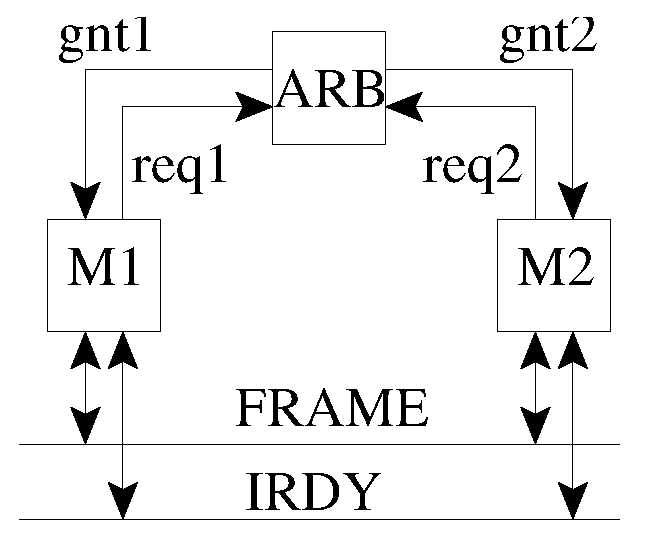
\includegraphics[scale=0.27]{pcistr.eps}}  % arindam: please do not delete this line. used for fig2ps
% \input{pcistr}}
% \subfigure[PCI Master Interface]{\label{pcistate}
\hspace{0.11in}
\subfigure[]{\label{pcistate}
% 
\includegraphics[scale=0.18]{pcistate.pstex}}  arindam: please do not delete this line. used for fig2ps
\begin{picture}(0,0)%

\includegraphics{pcistate.ps}%
\end{picture}%
\setlength{\unitlength}{1066sp}%
%
\begingroup\makeatletter\ifx\SetFigFont\undefined%
\gdef\SetFigFont#1#2#3#4#5{%
  \reset@font\fontsize{#1}{#2pt}%
  \fontfamily{#3}\fontseries{#4}\fontshape{#5}%
  \selectfont}%
\fi\endgroup%
\begin{picture}(6317,5739)(151,-5860)
\put(4951,-2761){\makebox(0,0)[lb]{\smash{\SetFigFont{8}{9.6}{\rmdefault}{\mddefault}{\updefault}{\color[rgb]{0,0,0}$\lnot$}%
}}}
\put(4276,-3511){\makebox(0,0)[lb]{\smash{\SetFigFont{8}{9.6}{\rmdefault}{\mddefault}{\updefault}{\color[rgb]{0,0,0}$\top$}%
}}}
\put(4276,-3886){\makebox(0,0)[lb]{\smash{\SetFigFont{8}{9.6}{\rmdefault}{\mddefault}{\updefault}{\color[rgb]{0,0,0}$\top$}%
}}}
\put(1276,-1861){\makebox(0,0)[lb]{\smash{\SetFigFont{8}{9.6}{\rmdefault}{\mddefault}{\updefault}{\color[rgb]{0,0,0}$\top$}%
}}}
\put(2476,-4786){\makebox(0,0)[lb]{\smash{\SetFigFont{8}{9.6}{\rmdefault}{\mddefault}{\updefault}{\color[rgb]{0,0,0}$\land$}%
}}}
\put(2401,-3061){\makebox(0,0)[lb]{\smash{\SetFigFont{8}{9.6}{\rmdefault}{\mddefault}{\updefault}{\color[rgb]{0,0,0}$\lnot$}%
}}}
\put(2251,-436){\makebox(0,0)[lb]{\smash{\SetFigFont{8}{9.6}{\rmdefault}{\mddefault}{\updefault}{\color[rgb]{0,0,0}$\lnot$}%
}}}
\put(1276,-1336){\makebox(0,0)[lb]{\smash{\SetFigFont{8}{9.6}{\rmdefault}{\mddefault}{\updefault}{\color[rgb]{0,0,0}$\lnot$}%
}}}
\put(526,-3961){\makebox(0,0)[lb]{\smash{\SetFigFont{8}{9.6}{\rmdefault}{\mddefault}{\updefault}{\color[rgb]{0,0,0}$\top$}%
}}}
\put(526,-4336){\makebox(0,0)[lb]{\smash{\SetFigFont{8}{9.6}{\rmdefault}{\mddefault}{\updefault}{\color[rgb]{0,0,0}$\top$}%
}}}
\put(226,-5611){\makebox(0,0)[lb]{\smash{\SetFigFont{8}{9.6}{\rmdefault}{\mddefault}{\updefault}{\color[rgb]{0,0,0}$\land$}%
}}}
\put(601,-5611){\makebox(0,0)[lb]{\smash{\SetFigFont{8}{9.6}{\rmdefault}{\mddefault}{\updefault}{\color[rgb]{0,0,0}$\lnot$}%
}}}
\end{picture}
}
\hspace{0.11in}
% \subfigure[Composition of two PCI master interfaces]{\label{pcicompstate}
\subfigure[]{\label{pcicompstate}
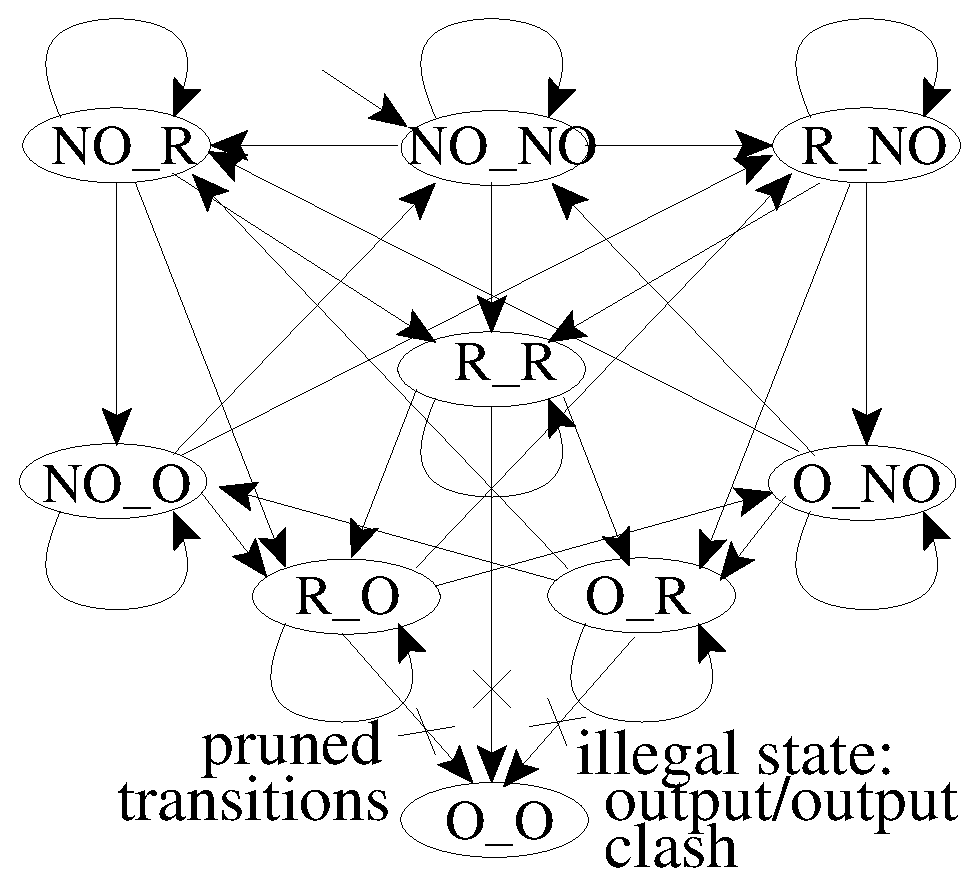
\includegraphics[scale=0.27]{pcicompstate.eps}} \\ % arindam: please do not delete this line. used for fig2ps
% \input{pcicompstate}}
% \subfigure[Token-ring NT interface]{\label{tokenringstate}
\subfigure[]{\label{tokenringstr}
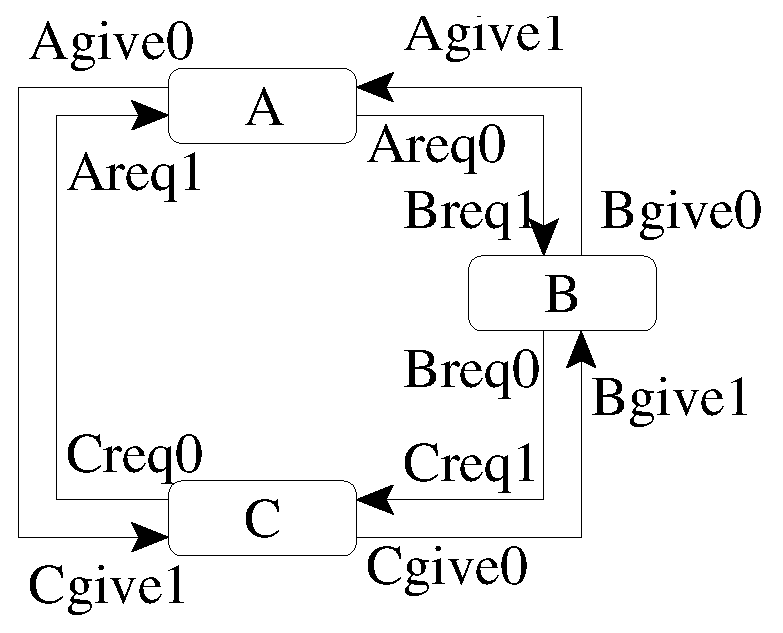
\includegraphics[scale=0.27]{tokenringstr.eps}}  % arindam: please do not delete this line; needed for fig2ps
% \input{tokenringstr}}
\hspace{0.15in}
\subfigure[]{\label{tokenringstate}
% 
\includegraphics[scale=0.18]{tokenringstate.pstex}}  arindam: please do not delete this line; needed for fig2ps
\begin{picture}(0,0)%

\includegraphics{tokenringstate.ps}%
\end{picture}%
\setlength{\unitlength}{1066sp}%
%
\begingroup\makeatletter\ifx\SetFigFont\undefined%
\gdef\SetFigFont#1#2#3#4#5{%
  \reset@font\fontsize{#1}{#2pt}%
  \fontfamily{#3}\fontseries{#4}\fontshape{#5}%
  \selectfont}%
\fi\endgroup%
\begin{picture}(7734,6264)(601,-5635)
\put(976,-4636){\makebox(0,0)[lb]{\smash{\SetFigFont{8}{9.6}{\rmdefault}{\mddefault}{\updefault}{\color[rgb]{0,0,0}$\top$}%
}}}
\put(901,-4186){\makebox(0,0)[lb]{\smash{\SetFigFont{8}{9.6}{\rmdefault}{\mddefault}{\updefault}{\color[rgb]{0,0,0}$\lnot$}%
}}}
\put(1276,-3661){\makebox(0,0)[lb]{\smash{\SetFigFont{8}{9.6}{\rmdefault}{\mddefault}{\updefault}{\color[rgb]{0,0,0}$\land$}%
}}}
\put(901,-2386){\makebox(0,0)[lb]{\smash{\SetFigFont{8}{9.6}{\rmdefault}{\mddefault}{\updefault}{\color[rgb]{0,0,0}$\lnot$}%
}}}
\put(901,-661){\makebox(0,0)[lb]{\smash{\SetFigFont{8}{9.6}{\rmdefault}{\mddefault}{\updefault}{\color[rgb]{0,0,0}$\lnot$}%
}}}
\put(901,-1036){\makebox(0,0)[lb]{\smash{\SetFigFont{8}{9.6}{\rmdefault}{\mddefault}{\updefault}{\color[rgb]{0,0,0}$\lnot$}%
}}}
\put(1501,239){\makebox(0,0)[lb]{\smash{\SetFigFont{8}{9.6}{\rmdefault}{\mddefault}{\updefault}{\color[rgb]{0,0,0}$\lnot$}%
}}}
\put(6976,-586){\makebox(0,0)[lb]{\smash{\SetFigFont{8}{9.6}{\rmdefault}{\mddefault}{\updefault}{\color[rgb]{0,0,0}$\top$}%
}}}
\put(6976,-961){\makebox(0,0)[lb]{\smash{\SetFigFont{8}{9.6}{\rmdefault}{\mddefault}{\updefault}{\color[rgb]{0,0,0}$\lnot$}%
}}}
\put(6151,-3361){\makebox(0,0)[lb]{\smash{\SetFigFont{8}{9.6}{\rmdefault}{\mddefault}{\updefault}{\color[rgb]{0,0,0}$\lnot$}%
}}}
\put(6976,-4186){\makebox(0,0)[lb]{\smash{\SetFigFont{8}{9.6}{\rmdefault}{\mddefault}{\updefault}{\color[rgb]{0,0,0}$\lnot$}%
}}}
\put(6976,-4561){\makebox(0,0)[lb]{\smash{\SetFigFont{8}{9.6}{\rmdefault}{\mddefault}{\updefault}{\color[rgb]{0,0,0}$\lnot$}%
}}}
\put(5476,-5536){\makebox(0,0)[lb]{\smash{\SetFigFont{8}{9.6}{\rmdefault}{\mddefault}{\updefault}{\color[rgb]{0,0,0}$\lnot$}%
}}}
\put(5101,314){\makebox(0,0)[lb]{\smash{\SetFigFont{8}{9.6}{\rmdefault}{\mddefault}{\updefault}{\color[rgb]{0,0,0}$\lnot$}%
}}}
\put(6526,314){\makebox(0,0)[lb]{\smash{\SetFigFont{8}{9.6}{\rmdefault}{\mddefault}{\updefault}{\color[rgb]{0,0,0}$\land$}%
}}}
\put(6976,-2761){\makebox(0,0)[lb]{\smash{\SetFigFont{8}{9.6}{\rmdefault}{\mddefault}{\updefault}{\color[rgb]{0,0,0}$\lnot$}%
}}}
\put(7126,-1561){\makebox(0,0)[lb]{\smash{\SetFigFont{8}{9.6}{\rmdefault}{\mddefault}{\updefault}{\color[rgb]{0,0,0}$\land$}%
}}}
\put(1801,-5461){\makebox(0,0)[lb]{\smash{\SetFigFont{8}{9.6}{\rmdefault}{\mddefault}{\updefault}{\color[rgb]{0,0,0}$\land$}%
}}}
\put(2176,-5536){\makebox(0,0)[lb]{\smash{\SetFigFont{8}{9.6}{\rmdefault}{\mddefault}{\updefault}{\color[rgb]{0,0,0}$\lnot$}%
}}}
\put(1501,-1711){\makebox(0,0)[lb]{\smash{\SetFigFont{8}{9.6}{\rmdefault}{\mddefault}{\updefault}{\color[rgb]{0,0,0}$\lnot$}%
}}}
\end{picture}
}

\caption{PCI and Token-ring Protocols 
\ref{pcistr} PCI Local Bus Structural Diagram
\ref{pcistate} PCI Master Interface
\ref{pcicompstate} Composite interface for two PCI Master Modules
\ref{tokenringstr} Token Ring Network Configuration
\ref{tokenringstate} Token-ring NT Interface
} 
\end{figure}

\begin{examp}{(PCI Bus)}
% The PCI bus protocol is well-known and widely used. 
We consider a PCI
bus configuration with two PCI-compliant master devices and a PCI
arbiter as shown in Figure~\ref{pcistr}.
Each PCI master device has an $gnt$ input and a $req$ output to
communicate with the arbiter, and a set of shared (read-write)
signals, the \verb+IRDY+ and the \verb+FRAME+, which are used to 
communicate with target devices. 
% The arbiter has the responsibility of deciding which master device is
% allowed to write to the shared signals in a bus cycle; more than one
% master writing simultaneously to the shared signals would be an error.
The arbiter ensures that at most one master device can 
write to the shared signals.
Figure~\ref{pcistate} shows a graphical description of the interface
representing a master device. The figure shows for each location, the
assumption (``a''), the guarantee (``g''), the set of inout variables 
that the interface writes to, and guarded transitions between locations.
Composing two such interfaces we obtain the interface shown in 
Figure~\ref{pcicompstate}. Location \verb+Owner_Owner+ is illegal
because both components write the shared variables \verb+FRAME+ and 
\verb+IRDY+. Input assumptions of locations \verb+Req_Req+, 
\verb+Owner_Req+ and \verb+Req_Owner+ are strengthened to make the 
illegal location unreachable.
Note that this propagates the PCI master's assumptions 
about its environment to an assumption on the behavior of the arbiter 
(which is the environment of the composite module): 
the arbiter should never assert \verb+gnt1+ (\verb+gnt2+) during or
after asserting \verb+gnt2+ (\verb+gnt1+),  until \verb+req2+
(\verb+req1+) is de-asserted at least once. \qed 
\end{examp}

\subsection{Properties of compatibility and composition} 

If $\mp$ and $\mq$ are composable Moore interfaces, we define their
{\em product\/} $\mp\oprod\mq$ by 
$\ovars_{\mp\oprod\mq} = \ovars_\mp \union \ovars_\mq$ and
$\ivars_{\mp\oprod\mq} = 
	(\ivars_\mp \union \ivars_\mq) \setm \ovars_{\mp\oprod\mq}$, 
and by letting 
$\oinit_{\mp\oprod\mq} = \oinit_\mp \und \oinit_\mq$, 
$\iinit_{\mp\oprod\mq} = \iinit_\mp \und \iinit_\mq$, 
$\otrans_{\mp\oprod\mq} = \otrans_\mp \und \otrans_\mq$, and 
$\itrans_{\mp\oprod\mq} = \otrans_\mp \und \itrans_\mq$.
\begin{comment} 
Intuitively, an environment for a Moore interface $\mp$ is an
interface that drives all free inputs of $\mp$, ensuring that all the
input assumptions are met. 
Precisely, we say that a Moore interface $\mq$ is an 
{\em environment\/} for a Moore interface $\mp$ if 
(i)~$\mp$ and $\mq$ are composable;
(ii)~$\mp\prod\mq$ is closed i.e., $\ivars_{\mp\oprod\mq} =
\emptyset$; 
(iii)~$\mp\prod\mq$ is non-blocking, i.e., $\iinit_{\mp\oprod\mq}$ is
satisfiable, and $\forall \ovars_{\mp\oprod\mq} . (\exists
\ivars_{\mp\oprod\mq})' . \itrans_{\mp\oprod\mq}$ holds; and 
(iv)~for all sequences $s_0, s_1, s_2, \ldots$ of
states in $\states[\vars_{\mp\oprod\mq}]$ with $s_0 \sat
\oinit_{\mp\oprod\mq}$ and $(s_k,s_{k+1}) \sat \otrans_{\mp\oprod\mq}$
for all $k \geq 0$, we have also that $s_0 \sat \iinit_{\mp\oprod\mq}$
and $(s_k,s_{k+1}) \sat \itrans_{\mp\oprod\mq}$ for all $k \geq 0$.
\end{comment}
%
Intuitively, an {\em environment\/} for a Moore interface $\mp$ is an
interface that drives all free inputs of $\mp$, ensuring that all the
input assumptions are met. 
Precisely, we say that a Moore interface $\mq$ is an 
environment for a Moore interface $\mp$ if $\mp$ and $\mq$ are
composable and closed (i.e., $\ovars_\mp \inters \ovars_\mq =
\emptyset$, and $\ivars_{\mp\oprod\mq} = \emptyset$), and if the
following conditions hold:  

%\vspace*{-1ex}

\begin{itemize}
\item {\em Non-blocking:\/} $\iinit_{\mp\oprod\mq}$ is satisfiable,
and $\forall \ovars_{\mp\oprod\mq} . (\exists \ivars_{\mp\oprod\mq})'
. \itrans_{\mp\oprod\mq}$ holds. 
\item {\em Legal:\/} for all sequences $s_0, s_1, s_2, \ldots$ of
states in $\states[\vars_{\mp\oprod\mq}]$ with $s_0 \sat
\oinit_{\mp\oprod\mq}$ and $(s_k,s_{k+1}) \sat \otrans_{\mp\oprod\mq}$
for all $k \geq 0$, we have also that $s_0 \sat \iinit_{\mp\oprod\mq}$
and $(s_k,s_{k+1}) \sat \itrans_{\mp\oprod\mq}$ for all $k \geq 0$.
\end{itemize}

%\vspace*{-1ex}

\noindent
Analogous definitions for product and environment can be given for
bidirectional interfaces. 
The following theorem states the main properties of compatibility and
composition of Moore interfaces; an analogous result holds for
bidirectional interfaces. 

\begin{theo}{(properties of compatibility and composition)}
The following assertions hold: 
%
\begin{enumerate}

\item % {\em Associativity:\/} 
Given three Moore interfaces $\mp$,
$\mq$, $\mr$, either $(\mp \| \mq) \| \mr$ and $(\mp \| \mq) \| \mr$
are both undefined (due to non-composability or incompatibility), or
they are both defined, in which case they are equal.

\item % {\em Compatibility as existence of environment:\/}
Given two composable Moore interfaces $\mp$ and $\mq$, we have that $\mp
\compat \mq$ iff there is an environment for $\mp\oprod\mq$. 

\item % {\em Composition and input assumptions:\/} 
Given two compatible Moore interfaces $\mp$ and $\mq$, 
and $\mr$ composable with $\mp\|\mq$, 
we have that $(\mp\|\mq) \compat \mr$ iff there is an environment 
for $\mp\oprod\mq\oprod\mr$. 

\end{enumerate}
\end{theo}

\noindent
The second assertion makes precise our statement that two interfaces
are compatible iff there is some environment in which they can work
correctly together. 
The third assertion states that composition does not unduly restrict
the input assumptions: checking compatibility with the composition
$\mp\|\mq$ amounts to checking compatibility with $\mp$ and $\mq$. 



\section{Refinement}

% Nice but long
\begin{comment} 
The refinement relation aims at formalizing the relation between
abstract and concrete versions of the same component, or between an
abstract component and its implementation.  
In the input-enabled (or pessimistic) setting, refinement is usually
defined as trace containment or simulation
\cite{Milner71}: this ensures that the set of output behaviors of the
implementation is a subset of that of the abstract component.  
However, such definitions are not be appropriate in a
non-input-enabled setting such as our interfaces: they would also
require that the set of legal inputs of the implementation is a
subset of that of the abstract component --- implying that the
implementation can be used in fewer environments than the abstract
component was designed for.
%
For example, if we adopted the classical definition, then the
component $\adder$ of Figure~\ref{fig-counter} would be refined by
a component $\strongadder$ having the same output transition relation, 
but that does not perform subtraction: precisely, with the 
{\em single\/} input guard {\tt [] true -> q1':=1}. 
%
As this example points out, refinement should be defined in a
contravariant fashion: the implementation should accept more inputs,
and produce fewer outputs, than the specification
\cite{luca-ia-01,luca-it-01}. 
\end{comment}

We define refinement as alternating simulation \cite{CONCUR98AHKV}:
roughly, a component $\mq$ refines $\mp$ (written $\mq \refi \mp$) if
$\mq$ can simulate all inputs of $\mp$, and if $\mp$ can simulate all
outputs of $\mq$.
Encoding the relation between the states of two Moore interfaces
$\mp$ and $\mq$ by a predicate $\rrp$, we can state the definition of
refinement as follows. 

\begin{defi}{(Refinement of Moore interfaces)}
\label{def-moore-ref} 
Given two Moore interfaces $\mp$ and $\mq$, 
% let $\avars = \ovars_\mp \setm \ovars_\mq$ be the set of ``private''
% variables of the specification. 
we have that $\mq \refi \mp$ if $\ivars_\mq \subs \ivars_\mp$ and 
$\ivars_\mp \inters (\ovars_\mp \union \ovars_\mq) = \emptyset$, 
and if there is a predicate $\rrp$ on $\vars_\mp \union \vars_\mq$
such that the following formulas are valid: 
%
\begin{eqalignno*}
\label{eq-moore-ref} 
  \iinit_\mp \und \oinit_\mq & \;\;\im \;\;
	\exists (\ovars_\mp \setm \ovars_\mq).
	(\iinit_\mq \und \oinit_\mp \und \rrp) \\
\rrp \und \itrans_\mp \und \otrans_\mq & \;\;\im\;\;
  \exists (\ovars_\mp \setm \ovars_\mq)'. 
	(\itrans_\mq \und \otrans_\mp \und \rrp') \hspace{2em} \qed 
\end{eqalignno*}
\end{defi}

% \noindent
% As an example, let $\adder'$ be the Moore interface obtained from
% $\adder$ by dropping the guarded command {\tt [] true -> q1':=1}, 
% and let $\adder''$ be the interface obtained from
% $\adder'$ by adding the guarded command {\tt q0 -> do':=do}. 
% Then, $\adder \refi \adder' \refi \adder''$, and the converse
% refinements do not hold. 

% \subsection{Implementation considerations} 

\noindent
As for normal simulation, there is a unique largest
refinement relation between any two Moore interfaces. 
% in fact, the union of two refinement relations is again a refinement
% relation. 
% In fact, indicating with 
% $\Psi_\tau(\rrp)$ and $\Psi_\theta(\rrp)$ the two formulas of 
% (\ref{eq-moore-ref}), it easy to see that if both 
% $\Psi_\tau(\rrp_1) \und \Psi_\theta(\rrp_1)$
% and
% $\Psi_\tau(\rrp_2) \und \Psi_\theta(\rrp_2)$, 
% then also 
% $\Psi_\tau(\rrp_1 \oder \rrp_2) \und \Psi_\theta(\rrp_1 \oder \rrp_2)$.
Hence, Definition~\ref{def-moore-ref}
provides an iterative algorithm for deciding refinement: 
let $\rrp_0 = \true$, and for $k \geq 0$, let 
%
\begin{equation} \label{eq-refi-comp} 
  \rrp_{k+1} = \rrp_k \und \forall (\vars_\mp \union \vars_\mq)' . 
  \bigl(\itrans_\mp \und \otrans_\mq \im 
  \exists (\ovars_\mp \setm \ovars_\mq)' . 
  (\itrans_\mq \und \otrans_\mp \und \rrp_k')\bigr).
\end{equation}
% 
Denoting with $\rrp_* = \lim_{k \go \infty} \rrp_k$ the fixpoint
(that again can be computed in a finite number of iterations), 
we have that $\mq \refi \mp$ if and only if (i)~$\ivars_\mq \subs
\ivars_\mp$ and  $\ivars_\mp \inters (\ovars_\mp \union \ovars_\mq) =
\emptyset$, and (ii)~$\iinit_\mp \und \oinit_\mq \;\im\; \exists 
(\ovars_\mp \setm \ovars_\mq) . (\iinit_\mq \und \oinit_\mp \und \rrp)$. 
In order to obtain an efficient implementation, we can again take
advantage for the computation of (\ref{eq-refi-comp}) of list
representations for the transition relations, and apply
image-computation techniques. 

Refinement of bidirectional  interfaces is defined similarly,
except that the refinement relation relates the locations of the two
interfaces, rather than the states. 
The definition is as follows. 

\begin{defi}{(Refinement of bidirectional  interfaces)}
Given two bidirectional  interfaces $\mp$ and $\mq$, $\mq$ refines
$\mp$ ($\mq \refi \mp$) iff there is 
% an alternating  simulation
% $\refi$ of $\mq$ by $\mp$ with $\hat{q}_{\mq} \refi \hat{q}_\mp$. 
% An alternating  simulation of $\mq$ by $\mp$ is 
a binary relation $\refi \subs Q_{\mq} \times Q_\mp$ 
such that $\hat{q}_{\mq} \refi \hat{q}_\mp$, 
and such that for all $q \refi p$ we have 
(i)~$\ivarsf_\mq(q) \subs \ivarsf_\mp(q)$, 
(ii)~$\ovarsf_{\mq}(q) \supseteq \ovarsf_\mp(p)$, 
(iii)~$\phi^i_{\mp}(p) \im \phi^i_\mq(q)$, 
(iv)~$\phi^o_\mq(q) \im \phi^o_\mp(p)$, 
(v)~for all $s \in \states[\ivarsf_\mp(p)]$ 
and all $t \in \states[\ovarsf_\mq(q)]$, 
if $s \sat \trel_\mp(p,p')$ and $t \sat \trel_\mq(q,q')$, 
then $q' \refi p'$. \qed 
\end{defi}

\noindent
We can check whether $\mq \refi \mp$ by adapting the classical
iterative refinement check \cite{Milner71}. 
We start with the total relation $\refi_0 = Q_\mq \times Q_\mp$, and
for $k \geq 0$, we let $\refi_{k+1}$ be the subset of $\refi_k$ such
that conditions~(i)--(v) hold, with $\refi_k$ in place of $\refi$ in
condition~(v). 
Once we reach $m \geq 0$ such that $\refi_{m+1} = \refi_m$, we have
that $\mq \refi \mp$ iff $\hat{q}_\mq \refi \hat{p}_\mq$. 
Since bidirectional interfaces are deterministic we can reduce
the refinement checking problem to graph reachability on the product
interface and hence $\mq \refi \mp$ can be decided in $O(|Q_\mq| \times
|Q_\mp|)$ time.

\begin{comment} 
%
% WARNING: old notation
%
\mynote{I cut out the algorithm here} 
\begin{algorithm}[ht]
\caption{Refinement Check for Stateful Bidirectional  Interfaces} \label{algo2}
\begin{algorithmic}[1]
\REQUIRE two stateful bidirectional  interfaces 
$F = (P_F,Q_F,\hat{q}_F,o_F,o^+_F,\phi_F,\psi_F,\delta_F)$ and
$F' = (P_{F'},Q_{F'},\hat{q}_{F'},o_{F'},o^+_{F'},\phi_{F'},\psi_{F'},\delta_{F'})$
\STATE Let $Prod_{F,F'} = F \circledast F' =$ a \emph{directed graph} 
$G(V_{Prod},E_{Prod})$ where 
$V_{Prod} = Q_F \times Q_{F'}$ and $E_{Prod} \subs V_{Prod} \times V_{Prod}$
such that $e = (v_1,v_2) \in E_{Prod}$ iff $v_1 = (q_1,q'_1)$, $v_2 = (q_2,q'_2)$
and $\exists$ valuations $i \in [P_F - o^+_F(q_1)]$, $o' \in [o_{F'}(q'_1]$ such that 
$\phi_F(q_1) @ i$ and $\psi_{F'}(q'_1) @ o'$ and $q_2 = \delta_F(q_1,i \uplus o')$
and $q'_2 = \delta_{F'}(q'_1,i \uplus o')$.
\STATE Let a state $v = (q,q')$ be an {\em error} state iff 
$(o_{F'}(q') \nsupseteq o_F(q)) \lor (o^+_{F'}(q') \nsubseteq o^+_F(q)) 
\lor (P_{F'} - o^+_{F'}(q') \nsubseteq P_F - o^+_F(q)) \lor 
(\phi_F(q) \nRightarrow \phi_{F'}(q')) \lor 
(\psi_{F'}(q') \nRightarrow \psi_F(q))$.
\IF {any error state is reachable from $(\hat{q}_F,\hat{q}_{F'})$ in 
$G(V_{Prod},E_{Prod})$}
\STATE $F'$ does not refine $F$
\ELSE
\STATE $F'$ refines $F$
\ENDIF
\end{algorithmic}
\end{algorithm}
\end{comment} 

\begin{examp}{(Token Ring)}
The IEEE 802.5 (Token Ring) is a widely used deterministic 
LAN protocol. Figure~\ref{tokenringstate} shows an interface modeling
a node that initially does not have the token. 
The same diagram with $T$ as initial state would 
represent a node that initially has the token. 
We call these two interfaces $NT$ and $T$, respectively.
The token ring components are connected in a cyclic network; each pair
of adjacent nodes communicate by $req$ and $gnt$ signals
(Figure~\ref{tokenringstr}). 
The $req$ signal flows clockwise, and is used to request the token; 
the signal $give$ flows counterclockwise, and is used to grant the token.
%
% As long
% as its $req$ input is de-asserted, it continues to hold the token. 
% When the token is requested, it goes into state $G$. %, where it may or may not 
% give the token to the requesting node immediately. When it decides to 
% give up the token, it asserts its $give$ output, sending the requesting 
% node into state $RR$ and itself going into state $RG$. When the 
% requesting node has got the token, it de-asserts its $req$ output, going 
% into state $T$, and this makes the other go into state $NT$, from which
% the sequence continues as before. The states $RG$ and $RR$ % are of
% technical importance only, to ensure that the token is not lost in transit.
% One would expect this protocol to fail if more than one node has the token 
% simultaneously. We verify this using interface compatibility checking.
% One would expect the protocol to work independent of the number of nodes
% in the network. We verify this using interface refinement.
%
The protocol fails if more than one node has the token simultaneously:
indeed, we can verify that two $T$ interfaces are not compatible,
while an $NT$ interface is compatible with a $T$ interface.  
Moreover, the protocol works for any number of participating nodes. 
To verify this, we check two refinements: 
first, an open-ring configuration consisting entirely of $NT$ nodes is a
refinement of the configuration consisting in just one $NT$ node; 
second, an open-ring configuration with any number of $NT$ nodes and
one $T$ node is a refinement of a configuration consisting in a single
$T$ node.   
Our implementation is able to perform the above compatibility and
refinement checks in a fraction of a second. \qed 
\end{examp}

% \begin{figure}
% \centering
% \subfigure[Token Ring NT interface]{\label{tokenringstate}
% 
\includegraphics[scale=0.20]{tokenringstate.pstex}}
% \hspace*{2em}
% \subfigure[Token Ring network]{\label{tokenringstr}
% 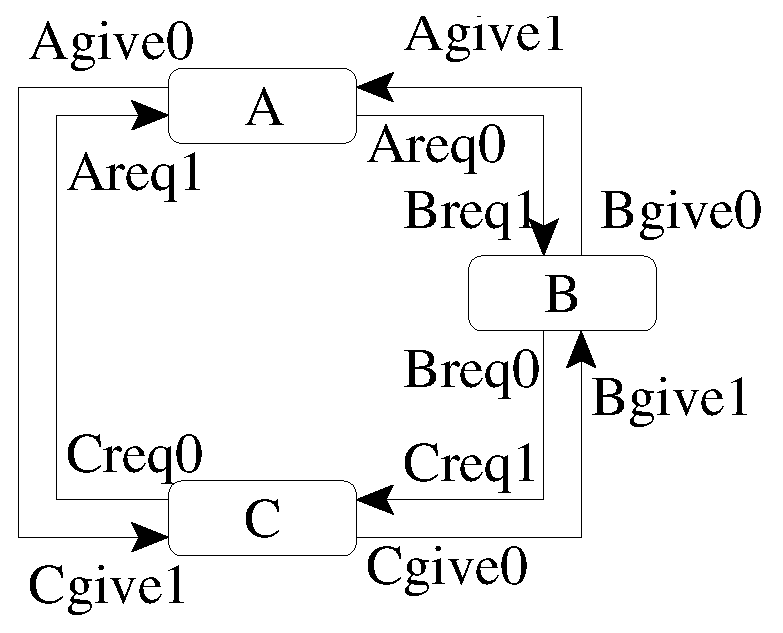
\includegraphics[scale=0.20]{tokenringstr.pstex}}
% \caption{Token ring protocol.} 
% \end{figure}

% The composition of two $T$ interfaces is found to be null. Thus our tool 
% verifies that two $T$ nodes are incompatible, as expected.
% It verifies that a network configuration with $1$ $T$ node and any number 
% of $NT$ nodes is a refinement of a network configuration with just 
% $1$ $T$ node, as expected.  
% Similarly a network configuration with any number of $NT$ nodes and no
% $T$ nodes is verified to be a refinement of a network configuration with 
% just one $NT$ node. 
% A network configuration with $k$ $NT$ nodes and no $T$ nodes is found 
% to be a refinement of a configuration with $n \leq k$ $NT$ nodes and 
% no $T$ nodes.
% This confirms the independence of the token ring protocol of the number
% of participating nodes. \qed

\noindent
The notion of refinement, in addition to implementation, captures also
substitutivity: if $\mq$ refines $\mp$, and $\mp$ is compatible with
the remainder $\mr$ of the design, then $\mr$ is also compatible with
$\mq$. 

\begin{theo}{(Substitutivity of refinement)}
Consider three bidirectional Moore or  bidirectional interfaces
$\mp, \mq, \mr$, such that $\mp\compat\mr$, and $\mq \refi \mp$. 
If $(\ovars_\mq \inters \ivars_\mr) \subs (\ovars_\mp \inters \ivars_\mr)$,
then $\mq\compat\mr$ and $(\mq \| \mr) \refi (\mp \| \mr)$. 
\end{theo}

\noindent
The  result has a proviso: all the variables that are output by $\mq$
and input by $\mr$ should also be output by $\mp$. 
If this were not the case, it would be possible for the additional
outputs of $\mq$ to violate the input assumptions of $\mr$.


% \subsection{Compositional verification} 

In compositional verification, one attempts to verify that an
implementation $\mp' \| \mq'$ refines a specificaton $\mp \| \mq$ 
by reasoning separately about $\mp'$ and $\mq'$. 
The simplest approach consists in proving that $\mp' \refi \mp$ and 
$\mq' \refi \mq$, but this seldom succeeds: usually, $\mp'$ refines
$\mp$ only in an environment (such as, hopefully, $\mq'$) that
provides it with the appropriate input. 
This approach has been refined by allowing the use of an environment
$\env_{\mp'}$ to restrict the possible inputs to $\mp$; 
then, in order to prove $\mp' \| \mq' \refi \mp \| \mq$, we show 
that both $\mp' \| \env_{\mp'} \refi \mp$ and 
$\mq' \| \env_{\mq'} \refi \mq$ hold. 
This approach is an instance of {\em assume-guarantee\/} reasoning 
\cite{Stark85,AbLa95,RM96,McMillan97}.
In \cite{RM96}, the environment $\env_{\mp'}$ is taken to be
$\mq$ (rule AG-SPEC):  
the specification itself is used to constrain the implementation; 
in \cite{concur99freddy}, $\env_{\mp'}$ is derived automatically from
$\mq$ (rule AG-IMPL), so that it reflects the implementation
(and symmetrically for $\env_{\mq'}$). 

In our interface formalisms we can restrict the possible inputs to a
component directly, without resorting to auxiliary environments, and
we can restate the above rules in a more direct and general way.
In the composition $\mp \| \mq$, the inputs of $\mp$ that are connected
to $\mq$ will only see output values that can be produced by $\mq$,
rather than arbitrary values; 
we can represent this constraint by an additional input restriction
for $\mp$. 
There are several possible ways of deriving these input restrictions 
from $\mq$;
for lack of space, we discuss here only 
an approach based on \cite{concur99freddy}. 
The approach, presented for Moore interfaces, can be readily adapted
to bidirectional A/G interfaces. 
Given two Moore interfaces $\mp$ and $\mq$, let $R$ be the predicate
defining the set of reachable states of $\mq$, computed as usual as
the fixpoint of the reachability computation $R_0 = \iinit_\mq \und
\oinit_\mq$, and $R'_{k+1} = R'_k \oder \exists \vars_\mq .  (R_k \und
\itrans_\mq \und \otrans_\mq)$, for $k \geq 0$.
%
Let $\avars$ be a set of variables that we wish to abstract away, 
let $\avars_\mq = (\vars_\mq \setm \vars_\mp) \inters \avars$
be the subset of those variables that appear in $\mq$ only, 
and let $\avars_\mp = \vars_\mq \setm (\vars_\mp \union \avars)$
be the variables of $\mq$ that we wish to include as inputs in $\mp$. 
%
Define $\adapt{\mp}{\mq}{\avars}$  to be the interface obtained
from $\mp$ by replacing $\ivars_\mp$ with 
$\ivars_\mp \union \avars_\mp$, 
%
by replacing $\iinit_\mp$ with 
$\iinit_\mp \und \exists \avars_\mq . \oinit_\mq$, 
%
and by replacing $\itrans_\mp$ with 
$\itrans_\mp \und \exists (\avars_\mq \union \avars_\mq') . 
(\reach(\vars_\mq,\oinit_\mq \und \iinit_\mq,\otrans_\mq \und
\itrans_\mq) \und \otrans_\mq)$.
%
Thus, the interface $\adapt{\mp}{\mq}{\avars}$ is obtained by
restricting the input assumptions of $\mp$ to reflect the possible
outputs of $\mq$. 
We can then state the following verification rule. 

\begin{theo}{(compositional refinement and adaptation)} 
\label{theo-comp-refi} 
For all interfaces $\mp, \mq, \mp', \mq'$ such that 
(i)~$\mp \compat \mq$, 
(ii)~$\mp'$ and $\mq'$ are composable (but not necessarily
compatible),
(iii)~$(\ovars_{\mp'} \inters \ivars_\mq) \subs (\ovars_\mp \inters \ivars_\mq)$,
and 
(iv)~$(\ovars_{\mq'} \inters \ivars_\mp) \subs (\ovars_\mq \inters \ivars_\mp)$,
and for all sets of variables $\avars_1$, $\avars_2$, $\avars_3$,
$\avars_4$, the following verification rule is valid: 
\[
  \frac{\adapt{\mp'}{\mq'}{\avars_1} \refi \adapt{\mp}{\mq}{\avars_2}; \hspace{1em} 
        \adapt{\mq'}{\mp'}{\avars_3} \refi \adapt{\mq}{\mp}{\avars_4}}{
	\mp' \compat \mq' \tand \ 
	\mp' \| \mq' \refi \mp \| \mq} \hspace{1em} (\mbox{\rm AG-INTF})
\]
\end{theo}

\noindent
In the rule, the input assumptions of both implementation and the
specification interfaces have been restricted to reflect their actual
environment. 
The proviso over the variables is necessary to ensure that the
compatibility of $\mp$ and $\mq$ implies that of $\mp'$ and $\mq'$,
once the refinement is proved. 
The theorem states a circular assume-guarantee principle: in fact,
$\adapt{\mp'}{\mq'}{\avars_1}$ is constructed using the fact that the
input assumptions of $\mq'$ are respected, even though the
compatibility of $\mp'$ and $\mq'$ is a conclusion of the rule, rather
than a premise; symmetrically for $\adapt{\mq'}{\mp'}{\avars_3}$.


It is easy to see that rule (AG-INTF) generalizes (AG-IMPL); to see
that it also generalizes (AG-SPEC), 
note that rule (AG-SPEC) can be restated as 
$(\mp' \refi \adapt{\mp}{\mq}{\emptyset}; 
  \mq' \refi \adapt{\mq}{\mp}{\emptyset})/
 (\mp' \| \mq' \refi \mp \| \mq)$.
In fact, our alternating notion of refinement requires the
implementation to match the specification only when the implementation
is subject to the same inputs as the specification. 
Hence, if we restrict the input assumptions of the specification (as
in $\adapt{\mp}{\mq}{\emptyset}$), we need to check that the
refinement holds only when the implementation $\mp'$ is subject to
similarly restricted inputs: thus, checking the alternating refinement  
$\mp' \refi \adapt{\mp}{\mq}{\emptyset}$ corresponds to checking the
regular refinement $\mp' \| \mq \refi \mp$ (where $\mp$, $\mq$, and
$\mp'$ are interpreted as regular modules, rather than interfaces). 
A symmetrical argument holds for the other premise. 







% \newpage
\bibliographystyle{plain}
\bibliography{luca}

\end{document}


